\subsection{M.2.6 Frequenza di pull request chiuse}
\begin{figure}[H]
    \centering
    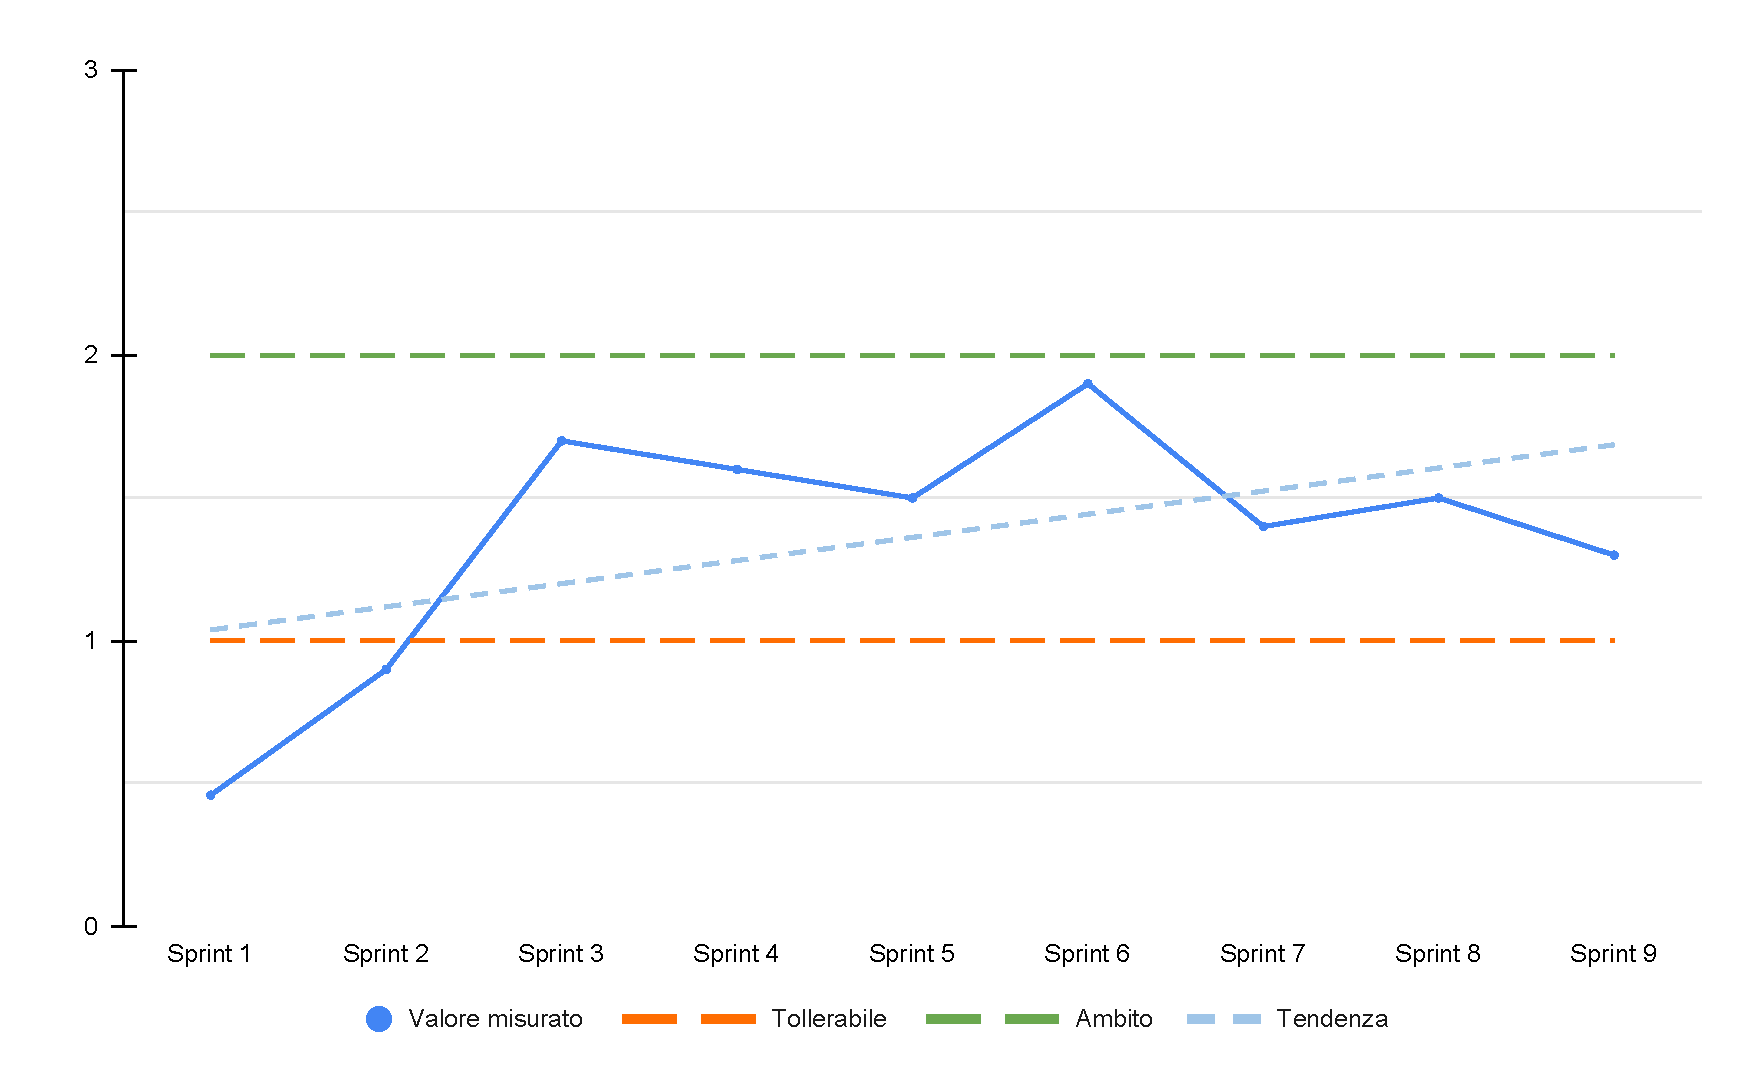
\includegraphics[width=0.8\textwidth]{assets/frequenza_pull_request.pdf}
    \caption{M.2.6 Frequenza di pull request chiuse}
\end{figure}

\par La frequenza di chiusura delle \glossario{pull request} vede un'andamento lineare: questo è dovuto al fatto che, nei primi \glossario{sprint}, il gruppo ha lavorato maggiormente sulla produzione di alcuni documenti, le quali modifiche o espansioni non richiedevano lo sviluppo di più pull request. Dagli \glossario{sprint} successivi, si è vista la necessità di aggiornare o espandere solo sezioni di quei documenti, il che ha portato alla necessità che il gruppo lavorasse separatamente a pezzi del documento, aumentando di conseguenza il numero di \glossario{pull request}. Un altro fattore che ha permesso l'aumento della media delle pull request chiuse è stato l'inizio dello studio di \glossario{txtai} e lo sviluppo del Proof of Concept, ai quali servivano \glossario{pull request} separate per l'avanzamento dei lavori.